%!TEX root = ./template-skripsi.tex
%-------------------------------------------------------------------------------
%                            BAB IV
%               		HASIL DAN PEMBAHASAN
%-------------------------------------------------------------------------------

\chapter{UJI COBA DAN HASIL UJI COBA}
	\section{Uji Coba}
		Dalam proses pengembangan aplikasi sesuai dengan SDLC, khususnya SDLC model spiral, uji coba dapat dikategorikan sebagai proses Evaluasi. Aplikasi yang telah selesai dikembangkan kemudian diujicobakan oleh beberapa ahli sebelum nantinya dirilis untuk masyarakat luas. Ahli yang akan menilai aplikasi ini adalah tiga dari empat ahli yang telah mengisi kuisioner identifikasi pada saat penelitian ini dimulai. Penulis mendatangi ketiga responden tersebut untuk melakukan uji coba dengan menggunakan ponsel milik penulis. Pertanyaan yang diajukan untuk para ahli berkisar tentang ketepatan dan kesesuaian konten yang dihasilkan oleh aplikasi. Komponen yang dinilai pada Uji Ahli tersebut adalah:
		\begin{itemize}
			\item Penilaian Konten Aplikasi
			\begin{enumerate}
				\item List Bahan yang tampil sesuai dengan resepnya
				\item List Cara Memasak yang tampil sesuai dengan resepnya
				\item Video YouTube yang diputar sesuai dengan Resepnya
				\item Takaran bahan tepat
				\item Langkah-langkah memasak yang ditampilkan tepat
			\end{enumerate}
			\item Penilaian Tampilan Aplikasi
			\begin{enumerate}
				\item Tulisan dapat dibaca dengan baik
				\item Elemen-elemen dalam aplikasi tertata dengan baik
				\item Ukuran gambar ideal (tidak terlalu besar atau kecil)
				\item Perpindahan antar halaman lancar
				\item Video YouTube dapat diputar dengan baik
				\item Wishlist dapat ditampilkan dengan baik
				\item Total Bahan pada Wishlist dapat ditampilkan dengan baik
				\item Total Harga pada Wishlist dapat ditampilkan dengan baik
				\item Total Rincian Harga pada Wishlist dapat ditampilkan dengan baik
			\end{enumerate}
			\item Penilaian Fungsionalitas Aplikasi
			\begin{enumerate}
				\item Resep dapat dimasukkan ke dalam Wishlist
				\item Resep dapat dihapus dari Wishlist
				\item Fitur Pencarian dapat mencari sesuai Bahan Resep
				\item Resep dapat dibagikan ke media sosial
			\end{enumerate}
		\end{itemize}
	
		Semua komponen penilaian tersebut akan dinilai dengan \textit{range} nilai antara 1 sampai 5 dengan perincian sebagai berikut:
		\begin{itemize}
			\item Nilai 1 - Sangat tidak setuju
			\item Nilai 2 - Tidak setuju
			\item Nilai 3 - Cukup
			\item Nilai 4 - Setuju
			\item Nilai 5 - Sangat setuju
		\end{itemize}
		\vspace{5cm}
		Data yang telah diperoleh kemudian dikalkulasikan dengan menggunakan sistem penilaian sebagai berikut:
		\begin{itemize}
			\item Nilai total\\
			Nilai ini adalah nilaitotal dari tiap pernyataan. Nilai total ini didapat dengan menggunakan persamaan sebagai berikut:\\
			$Nilai$ $total$ $=$ $jumlah$ $nilai$ $tiap$ $soal$
			\item Nilai rata-rata\\
			Nilai ini adalah nilai rata-rata dari tiap pernyataan dan didapat dengan menggunakan persamaan:\\
			$Nilai  rata-rata = \frac{nilai total}{jumlah partisipan}$
		\end{itemize}
	
	\section{Hasil Uji Coba Berdasarkan Aspek Penilaian}		
		Setelah dilakukan uji coba oleh tiga ahli di bidang kuliner dengan 18 item penilaian yang diajukan dengan sebaran 5 item penilaian konten, 9 item penilaian tampilan, dan 4 item penilaian fungsionalitas, penulis mengolah data hasil penilaian dari para ahli. Hasil diolah berdasarkan aspek penilaian yakni konten, tampilan, dan fungsionalitas.
		
		\subsection{Hasil Uji Coba Konten}
		
			\begin{table}[H]
				\centering
				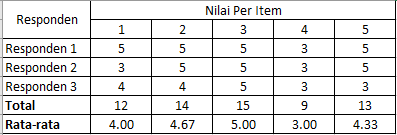
\includegraphics[width=0.6\textwidth]{gambar/new/konten_tabel}
				\caption{Tabel Nilai Hasil Uji Coba Konten}
				\label{tabel_konten}
			\end{table}
			Tabel \ref{tabel_konten} menunjukkan bahwa item penilaian ketiga, yakni Video YouTube yang diputar sesuai dengan resepnya, memiliki nilai tertinggi yaitu 5. Selanjutnya item penilaian kedua, yaitu list cara Memasak yang tampil sesuai dengan resepnya, menempati peringkat kedua dengan nilai 4,67. Item penilaian yang menempati peringkat ketiga dan keempat secara berturut-turut adalah item penilaian kelima dan pertama (langkah-langkah/cara-cara memasak yang ditampilkan tepat dan list bahan yang tampil sesuai dengan resepnya). Item penilaian dengan nilai terendah ditempati oleh item penilaian keempat dengan nilai 3 yakni takaran bahan tepat.  

		\subsection{Hasil Uji Coba Tampilan}

			\begin{table}[H]
				\centering
				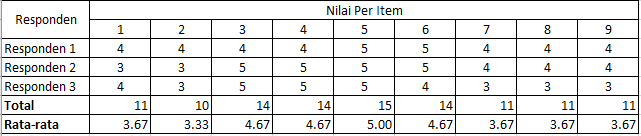
\includegraphics[width=1\textwidth]{gambar/new/tampilan_tabel}
				\caption{Tabel Nilai Hasil Uji Coba Tampilan}
				\label{tabel_tampilan}
			\end{table}
			Tabel \ref{tabel_tampilan} menunjukkan bahwa item penilaian kelima, yakni video YouTube dapat dimainkan dengan baik, memiliki nilai tertinggi yaitu 5. Sedangkan item penilaian kedua, yakni elemen-elemen dalam aplikasi tertata dengan baik, menempati posisi terbawah dengan nilai 3,33.
	
		\subsection{Hasil Uji Coba Tampilan}

			\begin{table}[H]
				\centering
				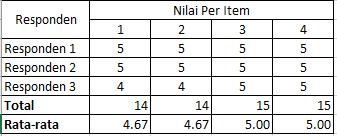
\includegraphics[width=0.6\textwidth]{gambar/new/fungsi_tabel}
				\caption{Tabel Nilai Hasil Uji Coba Fungsionalitas}
				\label{tabel_fungsionalitas}
			\end{table}
			Tabel \ref{tabel_fungsionalitas} menunjukkan bahwa item penilaian ketiga, yakni fitur pencarian dapat mencari sesuai bahan resep, dan item penilaian keempat, yakni resep dapat dibagikan ke media sosial, masing-masing memiliki nilai tertinggi yaitu 5. Sedangkan item penilaian pertama dan kedua, yakni resep dapat dimasukkan ke dalam \textit{wishlist} dan resep dapat dihapus dari \textit{wishlist}, masing-masing memiliki nilai terendah dengan nilai 4,67.			
	
	\section{Hasil Uji Coba Secara Keseluruhan}
		Dari data-data uji coba yang telah diolah berdasarkan aspek penilaian, dari segi konten, video YouTube yang diputar sesuai dengan resepnya, menempati peringkat teratas dalam proses uji coba. Dari segi tampilan, item penilaian video YouTube dapat dimainkan dengan baik juga menempati peringkat teratas. Sedangkan dari segi fungsionalitas, fitur pencarian dapat mencari sesuai bahan resep serta resep dapat dibagikan ke media sosial masing-masing juga menempati peringkat teratas. Hal ini menunjukkan bahwa video YouTube telah berhasil diimplementasikan secara baik dari segi konten maupun tampilan. Sedangkan fitur lain yang dapat berfungsi secara baik adalah fitur pencarian resep berdasarkan bahan serta fitur \textit{sharing} resep ke media sosial. Sejauh ini dapat disimpulkan bahwa implementasi YouTube kedalam aplikasi Android telah berhasil dilakukan.
		
		Sementara itu, para ahli juga memberikan beberapa masukkan kepada penulis untuk pengembangan aplikasi selanjutnya, yaitu:
		\begin{enumerate}
			\item Akan lebih baik apabila tampilan pada aplikasi ini tertata lebih baik lagi. Fungsi mencari bahan pada aplikasi ini sangat baik.
			\item Tambahkan fitur kapan bahan yang dimasak akan habis. 
			\item Kembangkan juga aplikasi untuk dapur restoran khususnya \textit{storing} bahan baku yang mencatat stok bahan di dapur.
			\item Berikan jumlah takaran yang lebih jelas lagi (beberapa bahan seperti gula dan garam tidak diberikan takaran yang spesifik)
			\item Berikan tips dan trik dalam memasak resep tersebut
			\item Memberikan keterangan pada tulisan berbahasa asing untuk menambah pengetahuan (contoh sudah diberikan pada kuisioner awal) 
		\end{enumerate} 
		
% Baris ini digunakan untuk membantu dalam melakukan sitasi.
% Karena diapit dengan comment, maka baris ini akan diabaikan
% oleh compiler LaTeX.
\begin{comment}
\bibliography{daftar-pustaka}
\end{comment}